%%%%%%%%%%%%%%%%%%%%%%%%%%%
% Fed Testimony Change Point Analysis
% Christopher Gandrud and Kevin Young
% 30 July 2014
%%%%%%%%%%%%%%%%%%%%%%%%%%%%

% !Rnw weave = knitr

\documentclass[a4paper]{article}\usepackage[]{graphicx}\usepackage[]{color}
%% maxwidth is the original width if it is less than linewidth
%% otherwise use linewidth (to make sure the graphics do not exceed the margin)
\makeatletter
\def\maxwidth{ %
  \ifdim\Gin@nat@width>\linewidth
    \linewidth
  \else
    \Gin@nat@width
  \fi
}
\makeatother

\definecolor{fgcolor}{rgb}{0.345, 0.345, 0.345}
\newcommand{\hlnum}[1]{\textcolor[rgb]{0.686,0.059,0.569}{#1}}%
\newcommand{\hlstr}[1]{\textcolor[rgb]{0.192,0.494,0.8}{#1}}%
\newcommand{\hlcom}[1]{\textcolor[rgb]{0.678,0.584,0.686}{\textit{#1}}}%
\newcommand{\hlopt}[1]{\textcolor[rgb]{0,0,0}{#1}}%
\newcommand{\hlstd}[1]{\textcolor[rgb]{0.345,0.345,0.345}{#1}}%
\newcommand{\hlkwa}[1]{\textcolor[rgb]{0.161,0.373,0.58}{\textbf{#1}}}%
\newcommand{\hlkwb}[1]{\textcolor[rgb]{0.69,0.353,0.396}{#1}}%
\newcommand{\hlkwc}[1]{\textcolor[rgb]{0.333,0.667,0.333}{#1}}%
\newcommand{\hlkwd}[1]{\textcolor[rgb]{0.737,0.353,0.396}{\textbf{#1}}}%

\usepackage{framed}
\makeatletter
\newenvironment{kframe}{%
 \def\at@end@of@kframe{}%
 \ifinner\ifhmode%
  \def\at@end@of@kframe{\end{minipage}}%
  \begin{minipage}{\columnwidth}%
 \fi\fi%
 \def\FrameCommand##1{\hskip\@totalleftmargin \hskip-\fboxsep
 \colorbox{shadecolor}{##1}\hskip-\fboxsep
     % There is no \\@totalrightmargin, so:
     \hskip-\linewidth \hskip-\@totalleftmargin \hskip\columnwidth}%
 \MakeFramed {\advance\hsize-\width
   \@totalleftmargin\z@ \linewidth\hsize
   \@setminipage}}%
 {\par\unskip\endMakeFramed%
 \at@end@of@kframe}
\makeatother

\definecolor{shadecolor}{rgb}{.97, .97, .97}
\definecolor{messagecolor}{rgb}{0, 0, 0}
\definecolor{warningcolor}{rgb}{1, 0, 1}
\definecolor{errorcolor}{rgb}{1, 0, 0}
\newenvironment{knitrout}{}{} % an empty environment to be redefined in TeX

\usepackage{alltt}
\usepackage{fullpage}
\usepackage[authoryear]{natbib}
\usepackage{setspace}
    \doublespacing
\usepackage[usenames,dvipsnames]{xcolor}
\usepackage{hyperref}
\hypersetup{
    colorlinks,
    citecolor=black,
    filecolor=black,
    linkcolor=cyan,
    urlcolor=cyan
}
\usepackage{dcolumn}
\usepackage{booktabs}
\usepackage{url}
\usepackage{tikz}
\usepackage{lscape}

\usepackage{todonotes}
\usepackage[utf8]{inputenc}

% Set knitr global options and load packages


%%%%%%% Title Page %%%%%%%%%%%%%%%%%%%%%%%%%%%%%%%%%%%%%%%%%%%%
\title{Creating Scrutiny Indicators: A Change Point Exploration of Congressional Scrutiny of the US Federal Reserve}

\author{Christopher Gandrud \\ {\emph{Hertie School of Governance}} \\ \& \\ Kevin Young \\ {\emph{University of Massachusetts, Amherst}}}
\IfFileExists{upquote.sty}{\usepackage{upquote}}{}
\begin{document}

\maketitle

%%%%%%% Abstract %%%%%%%%%%%%%%%%%%%%%%%%%%%%%%%%%%%%%%%%%%%%
\begin{abstract}

\noindent\emph{Draft. Comments welcome.}\footnote{Corresponding author: Christopher Gandrud, post-doctoral fellow at the Hertie School of Governance. Email: \href{mailto:gandrud@hertie-school.org}{gandrud@hertie-school.org}. \\ Thank to you Rebecca Kanter, Natalie McClung, and Brent Ramsey for research assistance. \\
All data and source code needed to reproduce this paper are available at: \url{http://dx.doi.org/10.5281/zenodo.11079}.}

We investigate trends in Congressional scrutiny of the US Federal Reserve from the late 1990s through 2012. Though independent, the Federal Reserve (the Fed) is accountable to legislative principles. Our aim is to develop indicators of high and low scrutiny from Congresspersons' behavior in committee hearings to gain an understanding of the political stressors that the Fed is under and which can be used in future research to examine how the Fed responds to pressures from legislators. We use change point analysis to estimate periods of high and low legislative scrutiny for both the US House of Representatives and Senate. Surprisingly, though the Senate has the power to approve Fed appointments, their scrutiny of the Fed does not seen to noticeably change over our observation period. The House Committee on Financial Services did noticeably increase its scrutiny of the Fed during the recent financial crisis. The paper also provides an introduction to how multivariate change point analysis could be used to estimate latent legislative scrutiny states.

\end{abstract}

\begin{description}
  \item [{\textbf{Keywords:}}] monetary policy, legislative oversight, change point analysis
\end{description}

Though politically independent, the US Federal Reserve (henceforth the Fed) is nonetheless subject to scrutiny by Congressional principles. Congress scrutinizes the Fed at both regular hearings, primarily the Fed governor's Semi-annual Report, as well as irregular hearings called by Congress to discuss specific issues such as the state of the housing market and financial regulatory changes. Previous studies of how legislatures influence independent monetary policy agents have often focused on \emph{de jure} transparency \citep[for example][]{Stasavage2003}. We create an indicator of (latent) legislative scrutiny, i.e. when Congress actually uses its \emph{de jure} transparency powers to examine the Fed's actions. To do this we conduct a change point analysis \citep{SenSrivastava1975, Killick2013, Matteson2014} of Congressional hearing transcripts to develop an indicator of time periods when there are higher and lower levels of Congressional scrutiny. We also begin to examine reasons behind scrutiny level changes. These indicators could be used in future work examining how Fed agents respond to legislative scrutiny by, for example, engaging with outside groups interest groups.

Previous research on Congressional scrutiny of the Fed has tended to focus not on Members' behavior in hearings, but instead on counts of proposed legislation that pertains to the Fed \citep[e.g.][]{Kettl1988}, many of which very rarely become law \citep{Binder2014}. Both hearings and bills indicate Congressional scrutiny. However, as Committees and their hearings are Congress' primary oversight tool \citep[][382]{oleszek2013} and proposed bills need to pass through these committees to become law, data from hearings is a more direct and relevant window onto day-to-day scrutiny. Bill counts also do not capture situations where Congress increases its scrutiny and the Fed successfully responds to head off legislative action.\footnote{See \url{https://github.com/christophergandrud/FedChangePointNote/tree/master/paper/data/Bills} for a comparison of the hearings-based scrutiny indicator and bill counts.}

In this paper we first discuss our sample of US Congressional hearings. We then give a brief overview of change point analysis and justify why it is a useful tool for determining states of high and low scrutiny. After this we present the results of change point analyses for four time-series derived from the Congressional hearings data: hearing frequency, the number of members present, formal letter correspondence between members of Congress and the Fed, and the frequency of laughter. We conduct a corresponding change point analysis on a number of macroeconomic indicators, especially indicators of the Fed's performance--inflation and unemployment--, to help understand when Congress changes its level of scrutiny.

\section{Congressional Hearings Data}

We gathered data on Congressional hearings--in both the Senate and the House of Representatives. We aimed to gather all of the hearing transcripts for (a) hearings where a Federal Reserve representative gave testimony and (b) any hearing of the US House of Representatives Committee on Financial Services (HCFS) and its predecessor the Committee on Banking and Financial Services, as well as the Senate Committee on Banking, Housing, and Urban Affairs (SCBUA) regardless of whether Fed testimony was given. Both of these committees have the normal responsibility for scrutinizing the Federal Reserve.

\subsection{Data Availability}

However, we were limited by data availability. We started by using the Federal Reserves' website\footnote{See: \url{http://www.federalreserve.gov/newsevents/default.htm}. Accessed Spring 2013 and Summer 2014.} to find information on all of the hearings at which its representatives gave testimony. At the time of data collection, the Fed's website has information on testimony made from 1996 through 2013. Also, only the prepared testimonies are available at this website. To gather full hearing transcripts we relied primarily on the US Government Printing Office (GPO) website.\footnote{See \url{http://www.gpo.gov/fdsys/browse/committeetab.action}. Accessed Spring 2013.} For most committees the GPO website only has full transcripts available from 2001 through 2012. We attempted to fill in missing transcripts with information available on individual committee's websites. Among the two committees we focused on, the HCFS had the most complete set of transcripts. Full HCFS hearing transcripts were available back to May 1997.\footnote{See: \url{http://financialservices.house.gov/archives/}. Accessed Spring 2013.} Unfortunately, the SCBUA archive website\footnote{See: \url{http://www.banking.senate.gov/public/index.cfm?FuseAction=Hearings.Home}. Accessed Spring 2013.} does not contain full hearing transcripts that we could have used to fill in transcripts missing from the GPO. So we decided to not include non-Fed SCBUA transcripts in our sample. As such we only have a complete corpus of full committee hearings transcripts (hearings with Fed testimony and not) for the HCFS.

\subsection{Observed Indicators}

We gathered four observable indicators of Congressional scrutiny from these transcripts. Possibly one of the closest observable indicators of latent scrutiny is the number of hearings that Fed representatives are asked to attend. If Congress holds more hearings in which it asks the Fed to send a representative in a given period of time, then they are scrutinizing it more. This is not a perfect measure of scrutiny, however, as the Fed may be asked to attend hearings scrutinizing not it, but another financial regulatory agency. As discussed earlier we also gather information on all of the hearings of the full HCFS. We will use these as a point of comparison.

We also look at Congress members' attendance at the hearings. Higher attendance provides a clear signal to Fed staff about Congress' interest in their activities. Again, this is not a perfect indicator of scrutiny. Lower attendance at any given meeting may, for example, result from unrelated issues such as scheduling conflicts. Attendance reporting was inconsistent across the committees. The HCFS had complete data on attendance. The SCBUA did not consistently report attendance, so we can not include it in our analyses.

Another indicator of scrutiny we gathered data on is formal letter correspondence between the Fed and members of Congress. As a government agency the Fed is required to respond formally to questions posed by Congress members not only in oversight hearings but also in written correspondence, which is submitted as part of the Congressional record as part of ``additional material submitted for the record''. For each instance in which the Fed appeared in Congress, we counted the number of such letters of correspondence. This may be a good indicator of Congressional scrutiny over the Fed for a variety of interrelated reasons. The Fed has good reason to take these letters as an indication of Congressional interest in its activities precisely because of the formal nature of the exchange. A Congressperson critical of the Fed is likely to ask questions that it wants a formal, written answer to on the record. In other instances, these letters constitute a follow-up to Congressional questioning that the Fed official could not answer to the satisfaction of a Congress member during the hearing. On this basis our expectation is that a spike in such letter correspondence represents a period of heightened scrutiny. Unfortunately, formal correspondence letters were not recorded in SCBUA transcripts.

Finally, we examine how many times instances of laughter were recorded in the testimony transcripts.\footnote{In all of our sets of transcripts instances of laughter are denoted ``[Laughter]''. Each instance does not indicate who or how many people are laughing.} We hypothesize that higher laughter counts indicate that the hearings have a more jovial non-adversarial atmosphere and the Fed has more reason to believe that Congresses is less concerned about their activities. For example, the highest hearing laughter count is from a February 2002 hearing where the Fed Chairman Alan Greenspan gave testimony at an annual SCBUA hearing on financial literacy.

\section{Methods: Change Point Analysis}

Our objective in this paper is to develop hearing-based indicators of periods when the Fed is under low or high scrutiny. A useful method for determining if there are changes in states through a time series is change point analysis. Change point analysis is a general term used to describe methods aimed at detecting changes in the ``statistical properties of a sequence of observations'' \cite[2]{Killick2013}. Imagine we have a series of data $y_{1:n} = (y_{1},\ldots,\: y_{n})$, for example, the monthly number of hearings.  We can say that a change has happened at a time $\tau \in \{1,\ldots,\:n-1\}$ in the data if the statistical properties, such as the means and variances, are different in $(y_{1},\ldots,\: y_{\tau})$ and $(y_{\tau},\ldots,\: y_{\tau})$. We can extend this logic to the study of series with multiple change points $m$ such that $\tau_{1:m} = (\tau_{1},\ldots,\:\tau_{m})$ and the data is broken into segments $m + 1$ \citep{Killick2012,Killick2013}. These segments could be periods of higher or lower legislative scrutiny of the Fed.

There are a number of different ways to estimate change points \cite[see][]{Killick2013,Matteson2014}. For our project we need a change point analysis method that (a) allows us to identify an unknown number of change points and (b) allows us to combine information from multiple observed variables to make inferences about latent scrutiny states. We want a method that allows us to estimate an unknown number of change points because we have no \emph{a priori} reason to assume that there is any fixed number of points at which the level of scrutiny changes. Also, we have no variable that directly captures the `legislative scrutiny' concept. It is instead a latent variable. The variables we do observe--hearing count, attendance, letter requests, and laughter--we expect to indicate in combination the level of scrutiny  Therefore we would like to combine information from all of these observed variables to understand the latent scrutiny level.

Matteson and James' \citeyearpar{Matteson2014} energy divisive hierarchical change point estimation algorithm allows us to achieve our two objectives. Their approach draws on Sz{\'e}kely and Rizzo's \citeyearpar{Szekely2005} work with hierarchical clustering. In particular they use the ``energy statistic'' method of determining statistical distances between probability distributions, e.g. the joint multivariate distributions of sequences of our observed Congressional hearing data. The time point where one sequence or cluster ends and another begins is a change point.

Of course, it may be that the the joint multivariate distributions of the estimated sequences are not in fact different, i.e. that every observation within the clusters are independent and identically distributed. In the language of hypothesis testing, this is the change point null hypothesis. Following \cite{Matteson2014} and \cite{Rizzo2010}, we examine this possibility using a permutation test with a maximum of 999 permutations to approximate the p-value for the hypothesis test. This produced stable estimates. We used the standard 0.05 p-value as a criteria for rejecting or failing to reject the null hypothesis, i.e. whether there is evidence for selecting a given change point or not.

One potential disadvantage of Matteson and James' change point method is that the minimum cluster size must be set \emph{a priori} \citeyearpar[11]{Matteson2014}. In other words, we need to tell the algorithm the minimum number of time points that may be between the change points. The minimum size generally needs to be larger if the distance between the probability distributions is small. We chose to use a minimum size of 24 months.\footnote{The \texttt{ecp} default is 30.} Across cases where change points could be estimated this size proved adequate to estimate statistically significant change points that were substantively meaningful.

\section{Scrutiny States}

The change point analyses by themselves only estimate clusters of time that are statistically different from their neighbors. To substantively interpret these results we need to compare the variables' distributions in the states with what we expect them to be in \emph{high} and \emph{low} scrutiny states. Our expectations are summarized in Table \ref{ExpectedTable}.

We expect that periods of high scrutiny will be characterized by frequent hearings, that are attended by many members, accompanied by many formal letter correspondences, and where there is little or no laughter. Periods of low scrutiny would have the opposite characteristics. See Table \ref{ExpectedTable} for a summary of our expectations about the scrutiny states.

\begin{table}
    \caption{Expected Relationship Between Hearing Indicators and Scrutiny States}
    \label{ExpectedTable}
    \begin{center}
        \begin{tabular}{l | c c}
            \hline
            & High Scrutiny & Low Scrutiny \\
            \hline \hline
            Hearings & frequent & infrequent \\[0.25cm]
            Attendance & high & low \\[0.25cm]
            Letter Correspondence & many & few \\[0.25cm]
            Laughter & infrequent & frequent \\
            \hline
        \end{tabular}
    \end{center}
\end{table}

\subsection{Interpreting the Change Points}

\begin{figure}
    \caption{Congressional Scrutiny of the Federal Reserve Change Point Analysis: Full US House Committee on Financial Services \emph{with} Federal Reserve Testimony}
    \label{fig:HouseFedCP}
\begin{knitrout}
\definecolor{shadecolor}{rgb}{0.969, 0.969, 0.969}\color{fgcolor}

{\centering 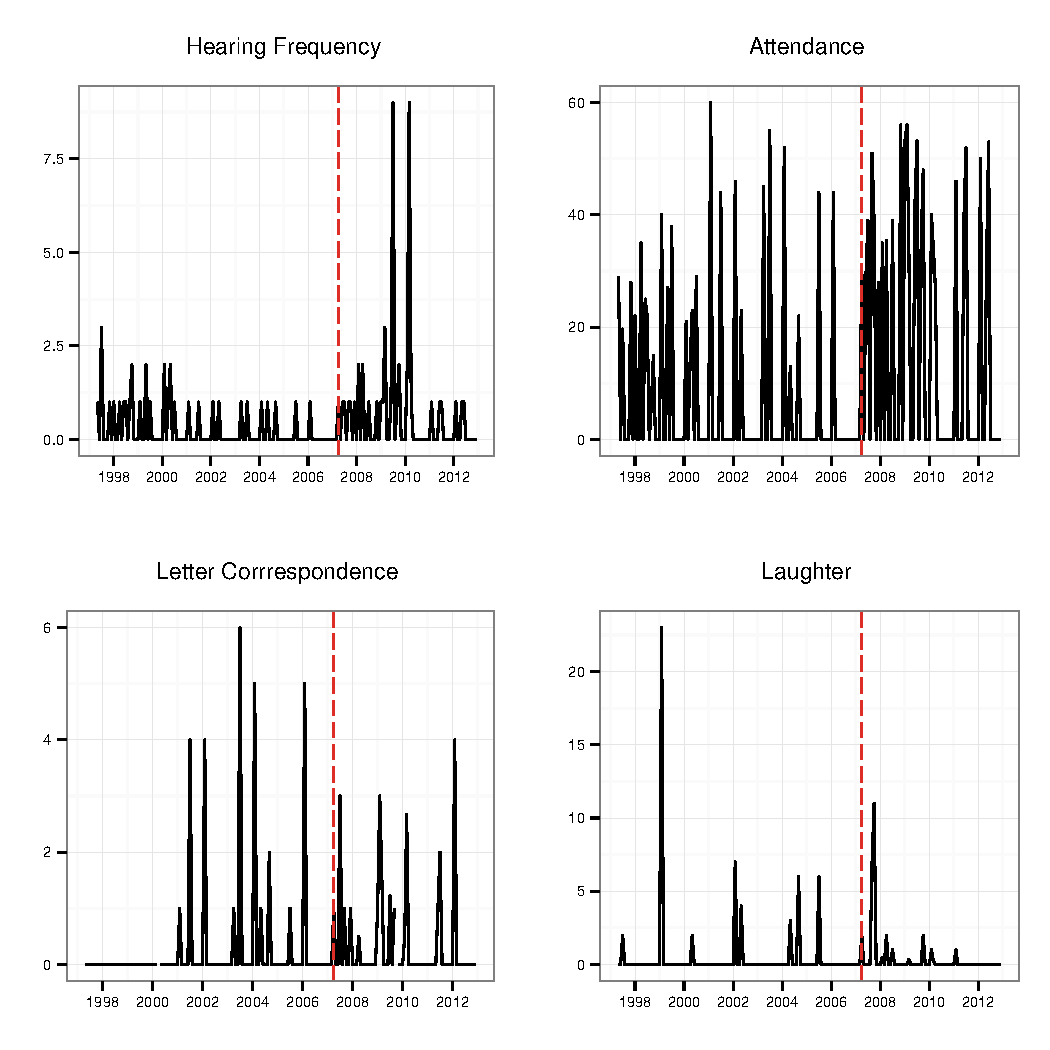
\includegraphics[width=0.95\linewidth]{figure/ScrutinyHouseFedCP} 

}



\end{knitrout}
{\scriptsize{The red horizontal dashed line signifies the estimated change points at the 95\% significance level from an analysis including both of the variables.\\
Minimum state width set at 24 months. \\
The data is aggregated on a monthly basis, i.e. observations represent monthly hearing counts or averages.}}
\end{figure}


\begin{figure}
    \caption{Congressional Scrutiny Change Point Analysis: Full US House Committee on Financial Services \emph{without} Federal Reserve Testimony}
    \label{fig:BaseNonFedCP}
\begin{knitrout}
\definecolor{shadecolor}{rgb}{0.969, 0.969, 0.969}\color{fgcolor}

{\centering 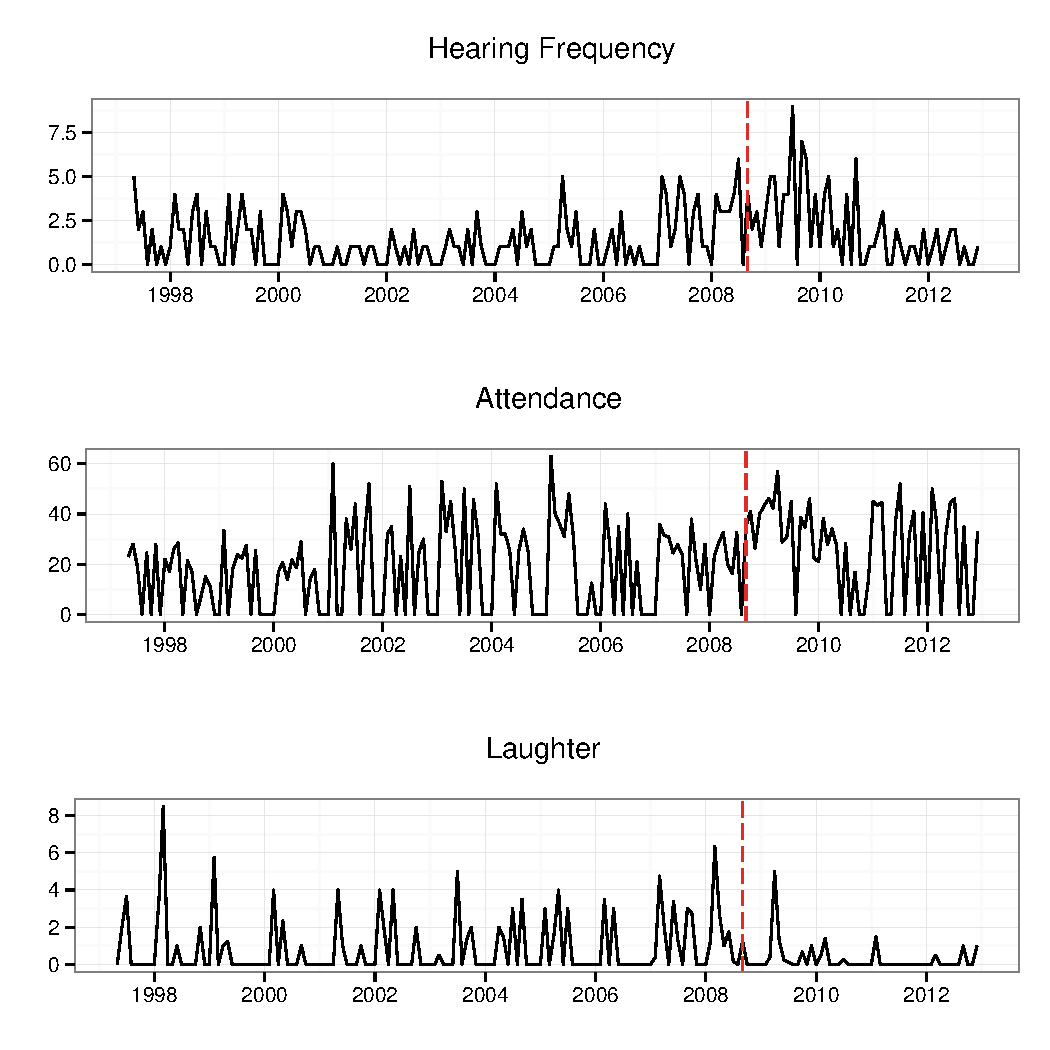
\includegraphics[width=0.8\linewidth]{figure/ScrutinyNonFedCP} 

}



\end{knitrout}
{\scriptsize{The red horizontal dashed line signifies the estimated change points at the 95\% significance level.\\
Minimum state width set at 24 months. \\
The data is aggregated on a monthly basis, i.e. observations represent monthly hearing counts or averages.}}
\end{figure}

We conducted three separate multivariate change point analyses to try to estimate Congressional scrutiny states. To implement these analyses we used a new function available at \url{https://gist.github.com/christophergandrud/5675688}. This function estimates the change points using the \emph{ecp} \citep{R-ecp} package for R \citep{CiteR} and plots the results compared to the original time series. The first analysis uses data from transcripts of hearings of the full HCFS where the Federal Reserve gave testimony. For comparison, we conduct an analysis on data from full HCFS hearings without Fed testimony. Obviously this analysis does not include letter correspondence with the Fed. Then we examine SCBUA hearings. As we discussed earlier, data is much more limited for the SCBUA. We have incomplete data on hearings without Fed testimony, especially before 2001. SCBUA transcripts also do not record formal letter correspondence and attendance. So our third change point analysis only includes data on the number of hearings by the full SCBUA and laughter at the hearings.

We aggregate our indicators by month. We measure hearing frequency as the number of hearings held in a month. Members attendance, correspondence, and laughter are aggregated using monthly means. Though some of these data are highly skewed--particularly laughter--there is not much difference between the monthly mean and median as most months only have no more than one hearing for a given committee. We have removed hearings that are held away from the Capital--so called ``field'' hearings--from the data. These meetings almost always have much lower attendance. Fewer than ten members usually attend. Fed representatives also almost never gives testimony at field hearings.

\begin{figure}
    \caption{Congressional Scrutiny Change Point Analysis: Full US Senate Committee on Banking, Housing, and Urban Affairs \emph{with} Federal Reserve Testimony}
    \label{fig:SenateFedCP}
\begin{knitrout}
\definecolor{shadecolor}{rgb}{0.969, 0.969, 0.969}\color{fgcolor}

{\centering 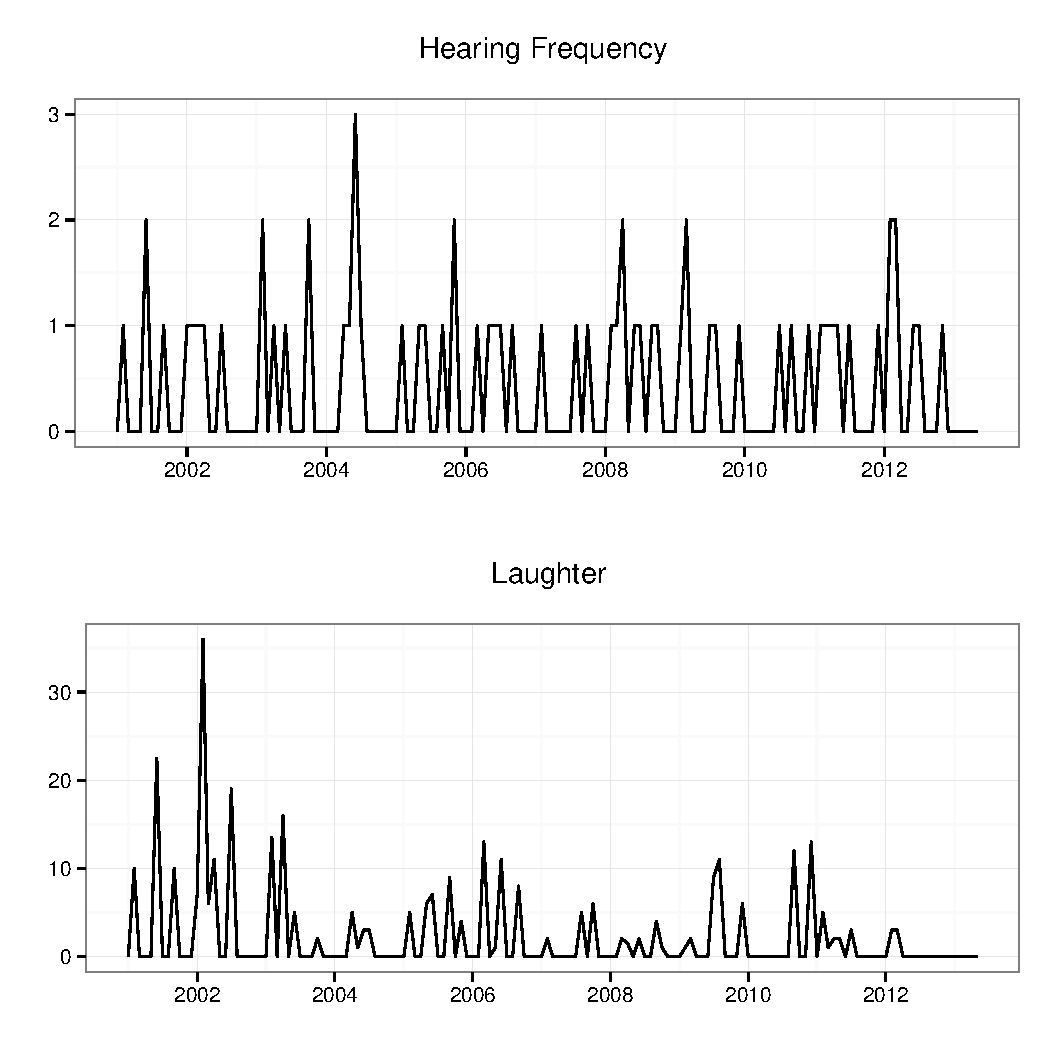
\includegraphics[width=0.8\linewidth]{figure/ScrutinySenate} 

}



\end{knitrout}
{\scriptsize{Note: no change points were estimated at conventional levels of statistical significance and using a wide range of minimum state widths.}}
\end{figure}

Figure \ref{fig:HouseFedCP} shows the change points (and underlying data from which they were estimated) for the HCFS when the Fed testified. Two change points were estimated at the 95\% significance level. The first in April 2007 and the second in May 2010. The scrutiny state that proceeded the first change point fairly closely conforms to our expectations about what a low scrutiny state would be. There were relatively infrequent hearings, moderate attendance, and fairly frequent laughter. Formal letter correspondence, despite our expectations does not seem to vary between this state and the others. The next state, between 2007 and 2010 largely corresponds to our expectations of a high scrutiny state. Hearings were very frequent, attendance was high, and laughter was fairly low, especially near the end of the period when the number of hearings was very high. The final state had characteristics of both high and low scrutiny states. The number of hearings was relatively low, but attendance was high and laughter was very low.

We estimated one change point in the data from the full HCFS hearings without Fed testimony. It was in February 2007 (see Figure \ref{fig:BaseNonFedCP}). This change point is similar to the one we estimated with the HCFS hearings including Fed testimony. The values of the indicator variables in the states are also similar. Hearings are relatively infrequent, attendance is moderate, as is laughter before the change point. Directly after the change point hearings become very frequent, attendance is moderate to high, and laughter is moderate. From about 2010, as with HCFS hearings with Fed testimony, hearings become more infrequent, attendance--with a brief lull--remains high, and laughter is very low. Despite these similarities, it's important to note that we did not estimate a statistically significant change point in 2010 in this data.

Increased scrutiny of the Fed appears to be closely related to scrutiny of other financial regulators, rather than being Fed specific. This finding is corroborated by \cite{SchonhardtBailey2012}. Using computer-assisted content analysis of the HCFS and SCBUA semi-annual monetary policy hearings during the recent financial crisis, she finds that a very large proportion of the discussion was about financial regulation generally, rather than monetary policy.

Figure \ref{fig:SenateFedCP} shows the (limited) data from full SCBUA hearings where the Fed gave testimony. We did not estimate any change points in the observation period using only hearing frequency and laughter. Using these limited indicators it does not appear that the SCBUA changed its level of scrutiny from mid-1997 through 2012. To a certain extent this finding may be the result of the SCBUA having relatively few members that are available to attend additional hearings. Nonetheless, this is very interesting given that the Senate, rather than the House, has the power to confirm presidents' Federal Reserve Board nominations.

\begin{table}
    \caption{Summary of Estimated Scrutiny States}
    \label{ObservedTable}
    \scalebox{0.9}{
        {\small{
        \begin{centering}
            \begin{tabular}{p{1.5cm}p{2.2cm}|p{2cm}p{2cm}p{2cm}p{2cm}p{2cm}}
                \hline
                &  & Number of Hearings  & Attendance  & Letter Correspondence  & Laughter  & Overall \tabularnewline
                \hline
                \hline
                HCFS with Fed  & Beginning-March 2007  & somewhat infrequent  & mixed  & mixed  & mixed to frequent  & Low \tabularnewline
                & April 2007-May 2010  & very frequent  & high  & mixed  & mixed  & High \tabularnewline
                & June 2010-End  & somewhat infrequent  & high  & mixed  & very infrequent  & Medium \tabularnewline
                \hline &  &  &  &  &  & \tabularnewline
                HCFS without Fed  & Beginning-January 2007  & infrequent to moderate  & moderate to high  &  & moderate to very low  & Low \tabularnewline
                & February 2007-End  & frequent to infrequent  & high  &  & moderate to very low  & High \tabularnewline
                \hline &  &  &  &  &  & \tabularnewline
                SCBUA with Fed  & Beginning to End  &  &  &  &  & Unchanging \tabularnewline
                &  &  &  &  &  & \tabularnewline
                \hline
            \end{tabular}
        \end{centering}
        }}
    }

    {\scriptsize{All interpretations are relative to the other states. \\
    `Beginning' and `End' denote the beginning and end of the observation period.}}
\end{table}

\section{Scrutiny States Compared to Economic States}

We conducted a similar change point analysis using economic data to get a better understanding of how key economic conditions may influence Congress to increase its scrutiny of the Federal Reserve. All of the data was gathered from the Federal Reserve Bank's Economic Data (FRED) database \citep{FRED}. The Fed's statutory obligations--as specified by the 1913 Federal Reserve Act--are to promote maximum employment and stable prices. Therefore we included measures of inflation and the unemployment rate. We also included a measure of general economic growth: the year on year percentage change of the gross domestic product per capita.\footnote{Inflation is measured as the year on year percent change in the seasonally adjusted personal consumption expenditures chain-type price index (FRED symbol: PCEPI). We used the unemployment indicator with the FRED symbol: U6RATE. Growth has FRED symbol: GDPC96.}

The results of the multivariate economic indicator change point analysis are illustrated in Figure \ref{fig:FullEconCP}. We estimate that there are 5 change points in the economic data from mid-1997 through 2012.\footnote{These dates were chosen to match the Congressional hearing data.} A number of the states correspond to relatively minor changes in the economic indicators. For example, the third state from late-2003 through late-2005 corresponds to a relatively minor increase in inflation and a similarly gradual fall in unemployment. Others, particularly the fifth state--between change points in October 2008 and October 2010--, correspond to fairly dramatic changes. The fifth state covers the 2008/2009 Global Financial Crisis.

When we compare the estimated HCFS scrutiny states to the economic states we see that the high scrutiny state between mid-2007 and mid-2010 roughly corresponds to economic state with the most severe changes in the observation period. Though the HCFS high scrutiny state for both the Fed and others--pre-dates the start of the most severe economic changes by about one year. Perhaps, using McCubbins and Schwartz's \citeyearpar{Mccubbins1984} terminology, Congress is responding to ``fire-alarms'' that indicate impending economic turmoil. The scrutiny of the Fed by the HCFS decreases a few months before the end of this severe economic changes state. Note that growth and inflation stabilize near their longer term trend before the end of the estimated severe economic crisis state ends. This is around the same point at which HCFS scrutiny of the Fed changes. Unemployment, however, remains high, declining only slowly. Reflecting this mixed economic condition, the HCFS entered a moderate scrutiny state when inflation and growth returned closer to normal, but unemployment remained high.

How big of a change may there need to be to inflation and other economic conditions for Congress to change its scrutiny on the Fed? There are two recessions in our sample (data on recessions is from FRED). The first was in 2001 following the Dotcom crash/the aftermath of the 9/11 terrorist attacks. The second ran from late 2007 until mid-2009 and resulted from the Global Financial Crisis. As we can see in the Figure \ref{fig:FullEconCP} the first recession was relatively mild compared to the second in terms of changes in inflation, unemployment and growth compared to the second. This indicates that Congress may only increase its scrutiny of the Fed and other financial policy bureaucrats when the economy is under extreme stress. It seems that Congress, specifically the HCFS, increases its scrutiny when the fire-alarms are very loud.

\begin{figure}
    \caption{Economic Indicator Change Point Analysis}
    \label{fig:FullEconCP}
\begin{knitrout}
\definecolor{shadecolor}{rgb}{0.969, 0.969, 0.969}\color{fgcolor}

{\centering 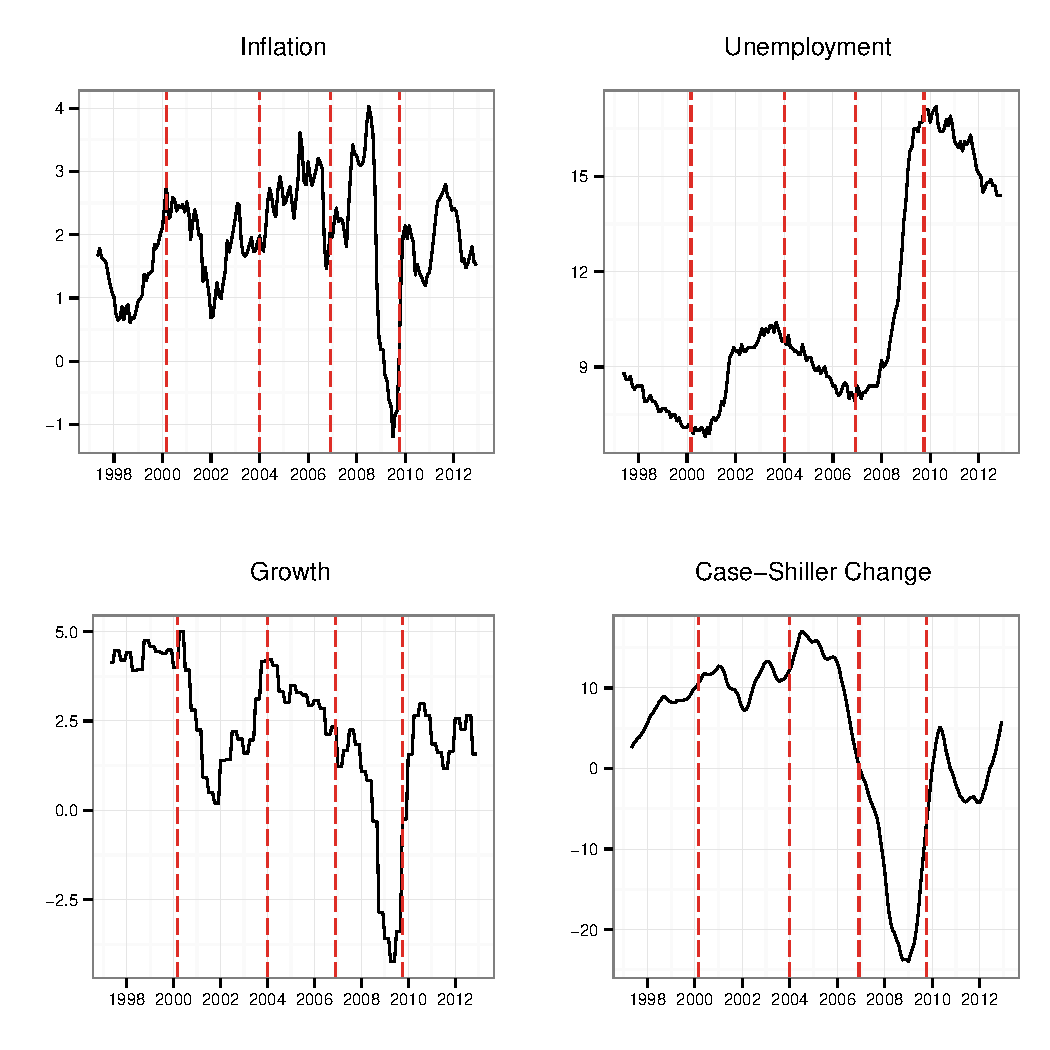
\includegraphics[width=0.8\linewidth]{figure/EconFullCP} 

}



\end{knitrout}
{\scriptsize{Red horizontal dashed lines signify the estimated change point at the 95\% significance level from an analysis including all of the variables.\\
Minimum state width set at 24 months. \\
Inflation is the percentage change in the chain-type personal consumption price index compared to the year before. Growth indicates GDP growth from the same quarter the year before. Unemployment is the unemployment rate for the month.}}
\end{figure}


\section{Discussion}

In this paper we have conducted a change point analysis of US Congressional hearings to develop indicators of scrutiny of the Fed. In addition we made investigated how economic conditions may affect scrutiny level changes. One of the ultimate goals of this research has been to develop indicators that can be used in future research to study interactions between the Fed and their legislative principles. The analysis also introduces political science researchers to the use of multivariate change point analysis for estimating legislative scrutiny states.

We found that changes in scrutiny--at least as suggested by the Congressional hearing transcript indicators--are different in the House Committee on Financial Services and Senate Committee on Banking and Urban Affairs. We found three Fed scrutiny states in the HCFS transcripts, but none in the SCBUA's. Though we initially expected there would be two types of scrutiny states--low and high--in the HCFS there seem to be three distinct types. From mid-1997 into 2007 there was a low scrutiny state, as we largely expected with our indicators. The one exception is that formal letter correspondence does not seem to correspond to changing scrutiny. The second state, which overlaps with a very severe economic crisis resulting from the 2008/2009 financial crisis, conforms to our expectations of being a high scrutiny state. The final HCFS state, however, seems to be between the two extremes. There are fewer hearings, but the hearings are well attended and almost no laughter occurs at them. Therefore, instead of using the change point analysis to create a simple dichotomous low/high legislative scrutiny variable it may be better to use the estimated change points to create a multinomial variable with distinct values for each cluster.

By comparing the estimated legislative scrutiny states to those estimated with key economic data, we have gained a better understanding of the conditions under which legislative scrutiny of the Federal Reserve changes. First, it seems that the HCFS increased its scrutiny of the Fed, and other financial agencies before the worst part of the recent financial crisis began. This indicates that the HCFS was responding to fire-alarms warning of crisis' onset. Second, scrutiny declined somewhat when inflation and growth stabilized close to pre-crisis levels, though unemployment remained high. Alongside this mixed economic state, we also saw a medium scrutiny state.


%%%%%%% Bib
\bibliographystyle{apsr}
\bibliography{MainBib,PaperPackages}

\end{document}
